\documentclass[fleqn,10pt]{physiome}
% Use option lineno for line numbers 
\usepackage{graphicx,amsmath,amssymb,dcolumn,xspace,euscript,xcolor}
\usepackage[version=4]{mhchem}
\usepackage{amsmath}
\usepackage{mathtools}
\usepackage{textcomp}
\usepackage{geometry}
\usepackage{amsfonts}
\usepackage{sidecap}
\usepackage{siunitx}
\usepackage{longtable}
\usepackage{multirow}
\articletype{Original}
%% Choose from Original, Retrospective, Review, Letter

\title{Reproducibility study of the modular and reusable model of epithelial transport in the proximal convoluted tubule}

\author[1][l.noroozbabaee@auckland.ac.nz]{Leyla Noroozbabaee}
\author[2]{Pablo J. Blanco}
\author[1]{Soroush Safaei}
\author[1]{David P. Nickerson}


\affil[1]{Auckland Bioengineering Institute, University of Auckland, New Zealand}
\affil[2]{National Laboratory for Scientific Computing, Petrópolis, Brazil}

%% The following lines can be omitted when submitting;
%% information will be added by editors
\publicationdate{14 June 2023}
\editor{Karin Lundengård}
\curator{Weiwei Ai}
\submitteddate{15 Dec 2022}
\citethisas{Noroozbabaee et al. (2023)\\A theoretical model of slow wave regulation using voltage-dependent synthesis of inositol 1, 4, 5-trisphosphate. Physiome.}{10.36903/physiome.21708176}

\begin{document}
\maketitle
\begin{abstract}
We describe here our implementation of a renal epithelial model as published in \cite{noroozbabaee2022modular}. The flexible and modular model we presented in \cite{noroozbabaee2022modular} can be adapted to specific configurations of epithelial transport. The model describes the cellular and subcellular mechanisms of the transporters, intracellular buffering, solute fluxes, and other processes. We provide free and open access to the Python implementation to ensure our multiscale proximal tubule model is accessible, enabling the reader to explore the model through configuring their own simulations, executing reproducibility tests and sensitivity analyses, and reusing the model in new work.
Here we present the reproduction of a selection of results from \cite{noroozbabaee2022modular}, providing readers with brief instructions on using the Python implementation to produce these results from the primary article.
\end{abstract}

\keywords{Proximal Tubule, Epithelial transport, Computational Model, Epithelial cell model, Python}
\primarypubs[10.36903/physiome.23499258]{Ref}{noroozbabaee2022modular}

\section{Introduction}
 In the primary article \citep{noroozbabaee2022modular}, we introduced a consistent, reproducible, and reusable proximal convoluted tubule (PCT) epithelial transport model. The comprehensive PCT epithelial model consists of cellular and lateral intercellular compartments located between luminal and peritubular solutions. The model includes fifteen solutes in each compartment and two impermeant species. The current work involves the mathematical curation of the model implementation in Python. A persistent workspace for this work is available under an open-source and permissive license at https://github.com/iNephron/W-PCT-E/releases/tag/v1.0.2.  
Here we demonstrate a quick instruction to reproduce figures related to the structural analysis section.

\section{Model description}
The comprehensive W-PCT-E model consists of cellular and lateral intercellular compartments between luminal and peritubular solutions. Figure~\ref{fig:Schematic_PCT} shows a schematic representation of PCT epithelium and features both configurations, in which cellular and lateral intercellular (LIS) compartments line the tubule lumen. Within each compartment, the concentration of species (i) is designated $C_{\alpha}(i)$, where ${\alpha}$ is lumen (M), lateral interspace (E), cell (I) or basal solution (S). Separating membranes are combinations of letters such as luminal cell membrane (lumen-cell membrane, MI), tight junction (ME), cell-lateral membrane (IE), interspace basement membrane (ES), or cell-basal membrane (IS). The order of the two letters indicates the positive direction of the mass flow. $J_{\alpha \beta}$ and $J_{\nu \alpha \beta}$ represent the solute flux and water flux, respectively, through the corresponding membrane; A is the related membrane surface area; V is the volume; E is the trans-epithelial potential difference. 
There are $14$ transporters (symporters, antiporters, complex transporters, and ATPases) that produce electrochemical fluxes in the current model.
\begin{figure}
    \centering
    \includegraphics[width=12cm]{Figure2.pdf}
    \caption{Schematic representation of the proximal convoluted tubule (PCT) epithelium, consisting of cell and lateral intercellular space, and a tubule model, in the way lumen is lined by epithelium \cite[Figure 2]{noroozbabaee2022modular}. }
    \label{fig:Schematic_PCT}
\end{figure}

\subsection{Modular Description}
The current Python code divides the mathematical W-PCT-E model into distinct components, which can be reused, eliminated or added to the model according to the desired experiments. Here we focus on the solute transport aspects of the model as listed in \autoref{Tab:components}. The reader is referred to the primary article for the complete description of all modules in the W-PCT-E model \citep{noroozbabaee2022modular}.

Each of these modules in  \autoref{Tab:components} is a Python model, enabling the researchers to reuse these components in their studies.

\begin{figure}[ht]
\centering
\includegraphics[width=7cm]{Figure3.pdf}
\caption{Proximal tubule cells showing coupled transport pathways and some ion channels within the luminal and peritubular cell membranes, \cite[Figure 3]{noroozbabaee2022modular}.}
\label{fig:Figure3}
\end{figure}

In this study, the designed experiments aim to investigate the model behaviour corresponding to either biological or, in some cases, extreme assumptions concerning the model configuration. Considering these assumptions, we can test the models' limitations, flexibility, or reliability. 
\begin{table}[]
\caption{Python Transport Modules (W$\_$PCT$\_$E$\_$Sim$\_$Fig.py. Here, all the equation numbers refer to the equation numbers in the primary paper.)}
\centering
\begin{tabular}{p{2.2cm} p{1.6cm} p{1.8cm} p{1.8cm} p{2.7cm} p{2.8cm}}
\hline
Compartment & Membrane & Stoichiometry & Equation &  Python Module & On-Off Parameter  \\
\hline
\multicolumn{6}{c}{Convective Transport}\\
Convective Flux & peritubular \& Apical & --- & Eq:(37) & def csf()& param$\_$csf\\
\hline
\multicolumn{6}{c}{Simple Diffusion}\\
Passive Flux & peritubular \& Apical & --- &  Eq(39-41)&  def goldman() & param$\_$goldman\\
\hline
\multicolumn{6}{c}{Simple Transport (Symporter)}\\
K\textsuperscript{+}-Cl\textsuperscript{-}& peritubular&  [1:1 ]& Eq:(42) & def k-cl()& param$\_$kcl\\

Na\textsuperscript{+}-glucose &  apical&  [1:1 ]& Eq:(43) & def sglt$\_$mi()& param$\_$sglt$\_$mi\\
Na\textsuperscript{+}-H\textsubscript{2}PO\textsubscript{4}\textsuperscript{-}&  apical&  [1:1 ]& Eq:(44) & def nah2po4$\_$mi()& param$\_$nah2po4$\_$mi\\

\multicolumn{6}{c}{Simple Transport (Antiporter)}\\
Na\textsuperscript{+}/H\textsuperscript{+}&  apical&  [1:-1 ]& Eq:(45) & def nah()& param$\_$nah$\_$mi\\
Na\textsuperscript{+}/NH\textsubscript{4}\textsuperscript{+}&  apical&  [1:-1 ]& Eq:(46) & def nanh4()& param$\_$nanh4$\_$mi\\

Cl\textsuperscript{-}/HCO\textsubscript{2}\textsuperscript{-} &  apical&  [1:-1 ]& Eq:(47) & def clhco2$\_$mi()& param$\_$clhco2$\_$mi\\
Cl\textsuperscript{-}/HCO\textsubscript{3}\textsuperscript{-} &  apical&  [1:-1 ]& Eq:(48) & def clhco3$\_$mi()& param$\_$clhco3$\_$mi\\
NHE3 & apical & \cite{weinstein_kinetically_1995} &  \cite{weinstein_kinetically_1995}& def nhe3() &param$\_$nhe3\\
\multicolumn{6}{c}{Complex Transport}\\
Na\textsuperscript{+}-3 HCO\textsubscript{3}\textsuperscript{-} & peritubular&  [1:3]& Eq:(49) & def na$\_$hco3()& param$\_$na$\_$hco3\\

Na\textsuperscript{+}-2 HCO\textsubscript{3}\textsuperscript{-}/Cl\textsuperscript{-}& peritubular&   [1:-1:2]& Eq:(50) & def na$\_$cl$\_$hco3()& param$\_$na$\_$cl$\_$hco3\\
\multicolumn{6}{c}{Active Transport}\\
H\textsuperscript{+}&   apical& -- & Eq:(53) & def h$\_$atp$\_$mi()& param$\_$mi$\_$h\\\\
Na\textsuperscript{+}/K\textsuperscript{+}-ATPS & peritubular&--& Eqs:(54-58)& def
nak$\_$atp()& param$\_$nak$\_$atp\\
\hline
\end{tabular}
 \label{Tab:components}
\end{table}

\section{Model status}
The current W-PCT-E model implementation in Python was executed using Python 3.9.0 [MSC v.1927 64 bit (AMD64)] on win32. The W-PCT-E model has been validated through the following experiments:
\begin{itemize}
   

 \item The W-PCT-E model reproducibility was tested by replicating some simulation experiments reported in \cite{Weinstein_1992} and \cite{Weinstein_2007}.

 \item The W-PCT-E model flexibility and reusability were tested by reproducing a simple model of Na+ transport in the mammalian urinary bladder to study the salt sensitivity, see \cite{latta_general_1984}.
\item Structural analysis of the W-PCT-E model validated the application of the model to the wide range of physiological perturbations.
\end{itemize}
\section{Model Computational Simulation}

For the W-PCT-E simulations, the $35$ nonlinear ordinary differential equations are solved using a finite difference numerical method for time discretisation along the Python solver ``scipy. optimise.root''. Evaluation of the model involves integrating the mass conservation equations from an initial time [t0 = 0 s] to a final time [tf = 2000 s] using small time increments [dt = 0.1 s]. The simulation time is chosen to ensure that a steady state is reached. To ensure your Python environment has the required Python modules used in these scripts, one needs to install all the Python requirements by performing ``pip install -r requirements.txt'' or as appropriate for your platform and Python environment.

\section{Model results}
 Here, we performed structural analysis on the W-PCT-E model to demonstrate its flexibility and explore its application to a range of physiological perturbations.
 To investigate the effect of each transporter in the W-PCT-E model on the overall behaviour, we performed experiments in which we individually inhibited each of the transporters and compared the total epithelial fluxes.
 
 Structural analyses were performed by inhibiting key transporters in different membranes, such as the \si{Na+/K+-ATPase} in the peritubular membrane or \si{SGLT}, \si{NHE3}, and \si{Na+-H2PO4} transporters in the apical membrane. The reproduction of structural analyses results of \citet{noroozbabaee2022modular} is given in Figures \ref{fig:Figure6}--\ref{fig:Figure8}, with the following sections providing instruction on how to use the associated Python codes to obtain these results.
 
To limit our focus on the structural analysis results and investigate the effect of different transporters in the W-PCT-E model [W$\_$PCT$\_$E$\_$Sim$\_$Fig.py], we define the model parameter ``Figure$\_$6$\_$7$\_$8 = 1''. It is important to mention that to stop the reproduction of the rest of the model simulation results; we need to make the following adjustment in the W-PCT-E model parameters: Figure$\_$4a = Figure$\_$4b = Figure$\_$4c = Figure$\_$5 = Figure$\_$9$\_$10 = 0. The version of the implementation associated with this manuscript has these settings, so no changes are needed. The following description defines the various parameters used throughout the [W$\_$PCT$\_$E$\_$Sim$\_$Fig.py] script to configure and execute the simulations required to produce the data presented here. No changes are required in the implementation. The resultant figures can be produced using the [Figures\_W\_PCT\_E.py] script by setting the desired figure parameter to $1$, with the figure numbering in the script aligned with the primary article (i.e., figures 6A, 6B, 7, 8A, and 8B).


\subsection{Inhibition of Peritubular (IS and IE) Transporters}
\label{Inhibition of Peritubular Transporters}
We separately eliminated the \ce{Na+}/\ce{K+}-ATPase and two symporters (\ce{K+}-\ce{Cl-} and \ce{Na+}-\ce{HCO3-}) on both the cell-basal and cell-lateral membranes and observed the resulting membrane fluxes and cellular concentrations. Inhibition of each transporter was accomplished by setting the coupling transport coefficient to zero. \autoref{fig:Figure6} presents the inhibition of basal and cell-lateral transporters -- this reproduces the results presented in Figure~6 of \cite{noroozbabaee2022modular}. On the first row in
each panel, we present four sets of results for four different configurations that depict
the total membrane fluxes for the following species: Na+, K+, Cl–, and Glucose. The total
membrane fluxes include all the membrane activities from five membranes. Panel (a) represents the original
full model (control configuration). Panel (b) illustrates the scenario due to the Na+-K+
pump elimination. Panel (c) corresponds to the K+- Cl – elimination scenario. Panel
(d) is for the inhibition of Na+-HCO3 – transporters. In the second row, we illustrate the cellular concentrations corresponding to the related configuration for the same species:
Na+, K+, Cl – , Glucose.

To obtain panel (a), we applied the default parameters [control configuration]. We ran the W-PCT-E model simulation [W$\_$PCT$\_$E$\_$Sim$\_$Fig.py] for the total time simulation of 2000 s and saved the related results in the python files to be used later by the Python file "Figures$\_$W$\_$PCT$\_$E.py".

To obtain panel (b), we eliminate the \si{Na+/K+-ATPase} by defining the "param$\_$sodium$\_$pumps = 0", while the rest of the system's parameters are the same as the default values. To reproduce panel (c), we eliminate the symporter \ce{K+}-\ce{Cl-}  by setting "param$\_$kcl = 0";
while we reset "param$\_$sodium$\_$pumps = 1".   Panel (d) illustrates the response of the W-PCT-E model in the case of elimination of \ce{Na+}-\ce{HCO3-} transporter by setting "param$\_$nahco3 =0"; while we reset "param$\_$sodium$\_$pumps = 1" and  "param$\_$kcl = 1". 

When we change the model configuration, we must ensure that the system's initial conditions correspond to physiological values. For this reason, we ran the model simulation for the first 500 s based on the control configuration. Then we applied the new configuration and continued the model simulation. We saved the results related to the fluxes in the python file: "Data$\_$Figure$\_$6A.py" and those related to solute concentrations in "Data$\_$Figure$\_$6B.py".






\subsection{Inhibition of Apical Membrane (MI) Transporters}
\label{Apical Membrane Transporters}
We separately eliminate the NHE3 antiporter and apical symporters (SGLT and \ce{Na+}-\ce{H2PO4-}). Then we study the behaviour of the W-PCT-E model by analysing the results for membrane fluxes and cellular concentrations relative to each scenario. Inhibition of each transporter was accomplished by setting the
coupling transport coefficient to zero. \autoref{fig:Figure8} presents the inhibition of apical membrane
transporters – this reproduces the results presented in Figure~8 of \cite{noroozbabaee2022modular}.

On the first row in each panel, we present four sets of results for four different configurations
that depict the total membrane fluxes for the indicated species.
Panel (a) represents the original
full model (control configuration). Panel (b) illustrates the scenario due to the  \si{NHE3} elimination. Panel (c) corresponds to the \ce{SGLT} elimination scenario. Panel
(d) is for the inhibition of \ce{Na+}-\ce{H2PO4-} – transporters. In the second row, we illustrate the cellular concentrations corresponding to the related configuration for the same species.

To obtain panel (a), we applied the default parameters [control configuration]. We ran the W-PCT-E model simulation [W$\_$PCT$\_$E$\_$Sim$\_$Fig.py] for the total time simulation of 2000 s.

To obtain panel (b), we eliminate the \si{NHE3} by defining the "param$\_$nhe3 = 0" while the rest of the system's parameters are the same as the default values. To reproduce panel (c), we eliminate the apical symporter \ce{SGLT}  by setting "param$\_$sglt$\_$mi = 0";
while we reset "param$\_$nhe3 = 1".   Panel (d) illustrates the response of the W-PCT-E model in the case of elimination of \ce{Na+}-\ce{H2PO4-} transporter by setting "param$\_$nah2po4$\_$mi = 0"; while we reset "param$\_$nhe3 = 1" and "param$\_$sglt = 1". 

We ran the model simulation for the first 500 s based on the control configuration. Then we applied the new configuration and continued the model simulation. We saved the results related to all the new configurations for the different fluxes in the python file: "Data$\_$Figure$\_$8A.py" and related results for the solute concentrations are saved in "Data$\_$Figure$\_$8B.py" to be used later by the Python file "Figures$\_$W$\_$PCT$\_$E.py".



\subsection{Total Epithelial Sodium Fluxes}

The first row in \cite[Figure 7]{noroozbabaee2022modular} represents the sodium fluxes for the full W-PCT-E model, considered the control version. In the second row, we illustrate the sodium fluxes due to the elimination of the \si{Na+/K+-ATPase}. And the third row corresponds to the elimination of NHE3. \autoref{fig:Figure7}  reproduces the results presented in Figure~7 of \cite{noroozbabaee2022modular}.

Panel (a) illustrates the different membrane fluxes. Panel (b) presents the epithelial sodium fluxes classified into convective, passive and electrochemical types. Panel (c) details the electrodiffusive activities into their segments: NHE3, SGLT, and \ce{Na+}-\ce{HPO4}. 

To reproduce \autoref{fig:Figure7}, we used the related results already produced by the previous simulations in \autoref{Inhibition of Peritubular Transporters} and \autoref{Apical Membrane Transporters}.  The results were collected in the python folder "Data$\_$Figure$\_$7.py".


\section{Discussion}
We have presented in \cite{noroozbabaee2022modular} what we believe to be a comprehensive and FAIR epithelial model for the PCT of the renal nephron.
Here, we aim to highlight the flexibility of the W-PCT-E model, as the user can have a better insight into the system behaviour due to the elimination or cooperation of transporters by simply turning them on or off.

Because of the flexibility of the W-PCT-E model, there is a future opportunity for similar analyses to describe the system behaviour due to the elimination of other transporters and their impact on the different solutes. 

The simulation experiments performed here aim to investigate the model behaviour corresponding to either biological or, in some cases, extreme assumptions concerning the model configuration. By considering these assumptions, we can test the models' limitations, flexibility, or reliability. 
In some cases, this pushed the boundaries of the biological system into the non-biological. These significant changes in configuration could, for example, generate an unrealistic stimulus in the model, which results in the model producing negative concentrations. To avoid the numerical error due to Eq. 52 in our primary paper (concerning its logarithmic nature), we added the if-else statements in the model implementation in the W$\_$PCT$\_$E$\_$Sim$\_$Fig.py file as shown below: 

\begin{verbatim}
def f_eps(c, z, v):    
    if c > 0 and c != 0: 
        return rte * np.log(c) + z * f * v * 1.e-6
    else:
        print('uy')
        return rte * np.log(abs(c)) + z * f * v * 1.e-6
   
\end{verbatim}
\newpage
\begin{figure}[h!]
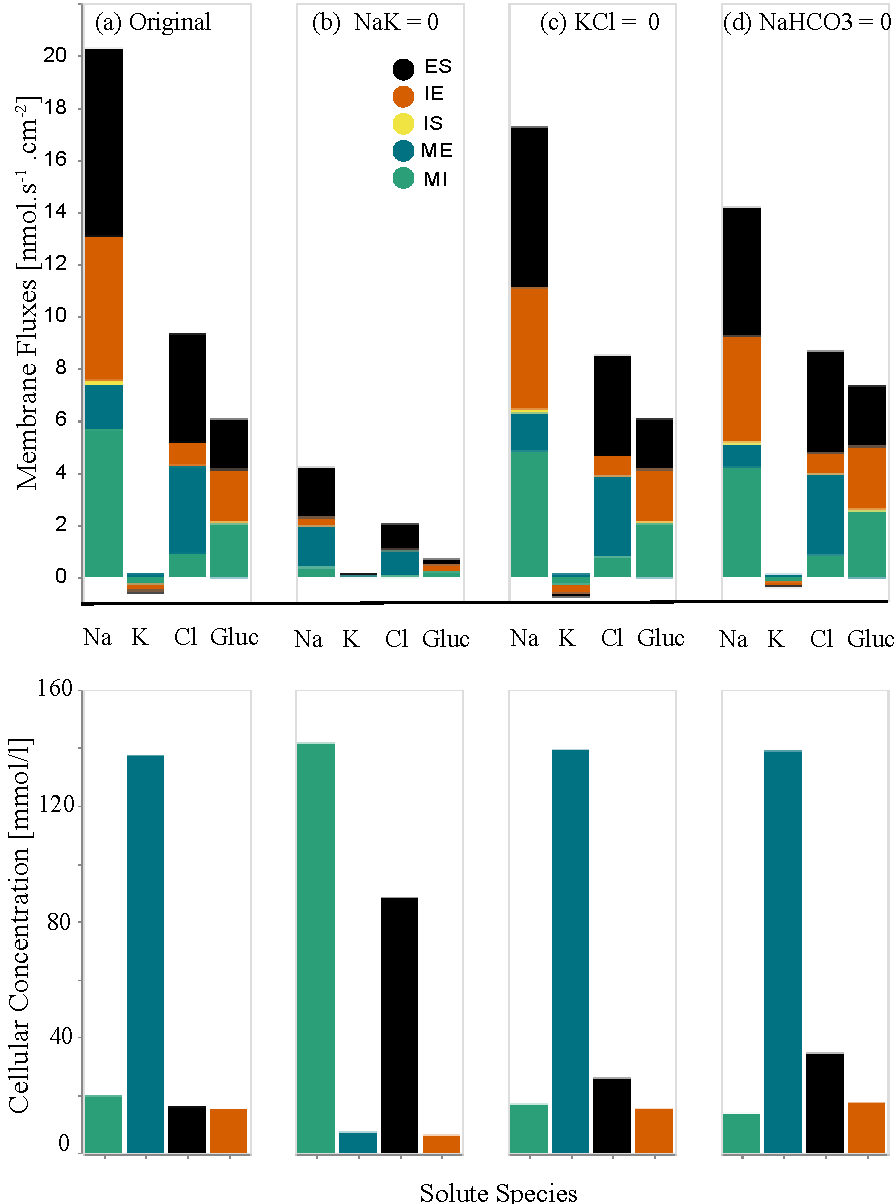
\includegraphics[width=1\linewidth]{Figure6.pdf}
\centering
\caption{Changes in the membrane fluxes (first row) and cellular concentrations (second row) due to the inhibition of transporters on the cell-basal and cell-lateral membranes, \cite[Figure 6]{noroozbabaee2022modular}.}
\label{fig:Figure6}
\end{figure}
\begin{figure}[h!]\centering
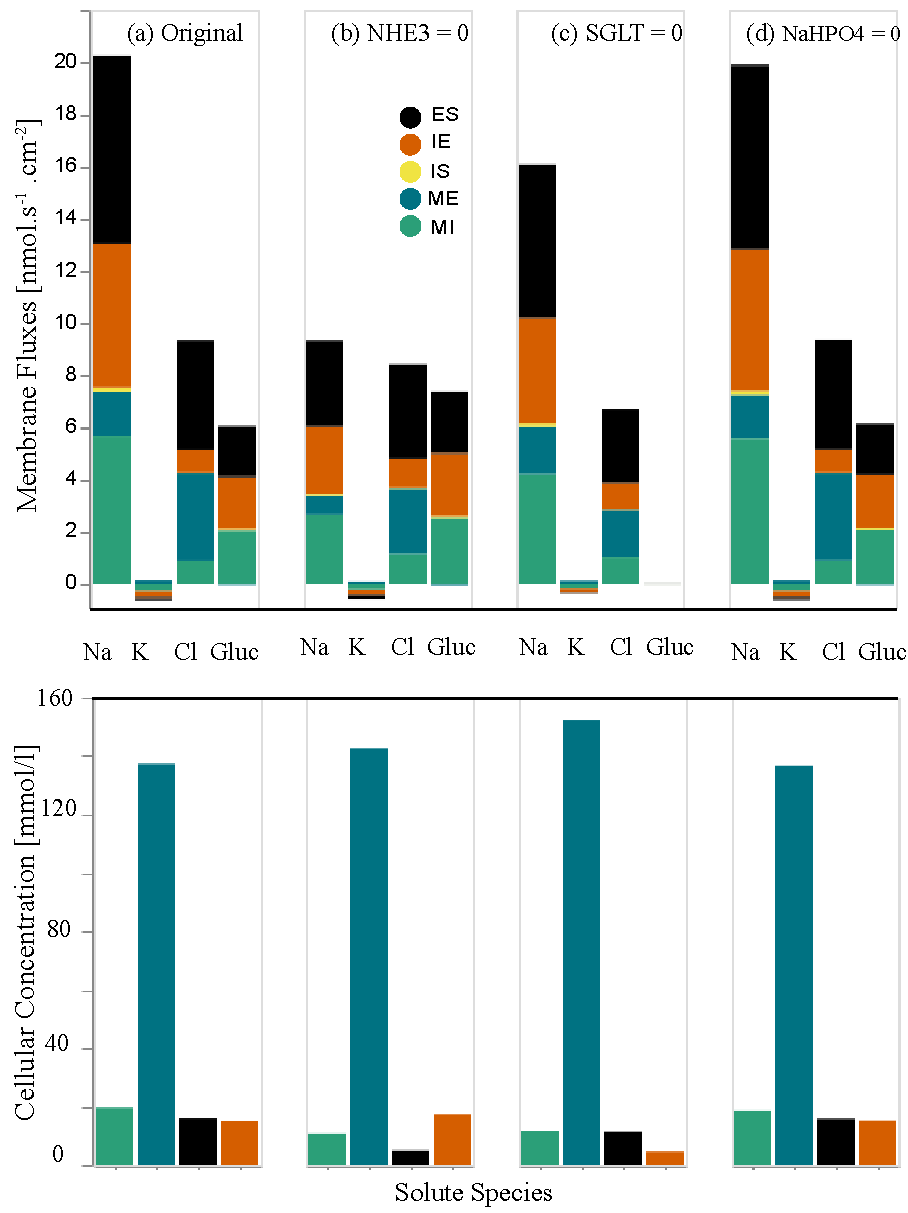
\includegraphics[width=1\linewidth]{Figure8.pdf}
\caption{Changes in the membrane fluxes (first row) and cellular concentrations (second row) due to the inhibition of transporters on the apical cell membrane, \cite[Figure 8]{noroozbabaee2022modular}.}
\label{fig:Figure8}
\end{figure}
\clearpage 
\pagebreak
\newpage

\begin{figure}[h!]
\includegraphics[width=1\linewidth]{Figure7.pdf}
\centering
\caption{Total epithelial sodium fluxes and the contribution of various sodium flux types, \cite[Figure 7]{noroozbabaee2022modular}. }
\label{fig:Figure7}
\end{figure}


% % Functional implications of the sex differences in transporter
% \parindent 0cm
% \bibliography{W_PCT_epithelial_bib.bib}
% % \bibliography{W-PCT-E-bib}


% \end{document}


\bibliography{Ref}

\end{document}